\documentclass[10pt]{beamer}\usepackage[]{graphicx}\usepackage[]{xcolor}
% maxwidth is the original width if it is less than linewidth
% otherwise use linewidth (to make sure the graphics do not exceed the margin)
\makeatletter
\def\maxwidth{ %
  \ifdim\Gin@nat@width>\linewidth
    \linewidth
  \else
    \Gin@nat@width
  \fi
}
\makeatother

\definecolor{fgcolor}{rgb}{0.345, 0.345, 0.345}
\newcommand{\hlnum}[1]{\textcolor[rgb]{0.686,0.059,0.569}{#1}}%
\newcommand{\hlstr}[1]{\textcolor[rgb]{0.192,0.494,0.8}{#1}}%
\newcommand{\hlcom}[1]{\textcolor[rgb]{0.678,0.584,0.686}{\textit{#1}}}%
\newcommand{\hlopt}[1]{\textcolor[rgb]{0,0,0}{#1}}%
\newcommand{\hlstd}[1]{\textcolor[rgb]{0.345,0.345,0.345}{#1}}%
\newcommand{\hlkwa}[1]{\textcolor[rgb]{0.161,0.373,0.58}{\textbf{#1}}}%
\newcommand{\hlkwb}[1]{\textcolor[rgb]{0.69,0.353,0.396}{#1}}%
\newcommand{\hlkwc}[1]{\textcolor[rgb]{0.333,0.667,0.333}{#1}}%
\newcommand{\hlkwd}[1]{\textcolor[rgb]{0.737,0.353,0.396}{\textbf{#1}}}%
\let\hlipl\hlkwb

\usepackage{framed}
\makeatletter
\newenvironment{kframe}{%
 \def\at@end@of@kframe{}%
 \ifinner\ifhmode%
  \def\at@end@of@kframe{\end{minipage}}%
  \begin{minipage}{\columnwidth}%
 \fi\fi%
 \def\FrameCommand##1{\hskip\@totalleftmargin \hskip-\fboxsep
 \colorbox{shadecolor}{##1}\hskip-\fboxsep
     % There is no \\@totalrightmargin, so:
     \hskip-\linewidth \hskip-\@totalleftmargin \hskip\columnwidth}%
 \MakeFramed {\advance\hsize-\width
   \@totalleftmargin\z@ \linewidth\hsize
   \@setminipage}}%
 {\par\unskip\endMakeFramed%
 \at@end@of@kframe}
\makeatother

\definecolor{shadecolor}{rgb}{.97, .97, .97}
\definecolor{messagecolor}{rgb}{0, 0, 0}
\definecolor{warningcolor}{rgb}{1, 0, 1}
\definecolor{errorcolor}{rgb}{1, 0, 0}
\newenvironment{knitrout}{}{} % an empty environment to be redefined in TeX

\usepackage{alltt}

\usepackage[T1]{fontenc}
\usepackage[french]{babel}
\usepackage{amsmath}
\usepackage{amssymb}
\usepackage{booktabs}
\usepackage{siunitx}
\usepackage{multirow}

% \usetheme{Madrid}

\usetheme{CambridgeUS}
\usecolortheme{spruce}

\setbeamertemplate{navigation symbols}{}
\setbeamertemplate{caption}[numbered]{}% Number float-like environments

% Make toc bullets dark green to match the theme
\setbeamercolor{section number projected}{bg=green!40!black,fg=white}
\setbeamercolor{subsection number projected}{bg=green!40!black,fg=white}
% Do the same for bullets in itemize/enumerate environments
\setbeamercolor{item projected}{bg=green!40!black,fg=white}
\setbeamercolor{subitem projected}{bg=green!40!black,fg=white}
\setbeamercolor{subsubitem projected}{bg=green!40!black,fg=white}
% Change the color of "Figure X -" in captions
\setbeamercolor{caption name}{fg=green!40!black}

\renewcommand{\frenchtablename}{Tableau}


\renewcommand{\frenchtablename}{Tableau}

\title[S2-APP6: Analyse d'EQ analogique]{S2-APP6: Analyse d'un égaliseur analogique}
\author[Benjamin Chausse \& Cédrick Pelchat]{
  Benjamin Chausse (chab1704)\\
  Cédrick Pelchat (pelc1105)
}
\institute[UDS]{Université de Sherbrooke}
\date{\today}
% \logo{\includegraphics[height=2cm]{logo.pdf}}

\AtBeginSection[]{
\begin{frame}
  \vfill
  \centering
  \begin{beamercolorbox}[sep=8pt,center,shadow=true,rounded=true]{title}
    \usebeamerfont{title}\insertsectionhead\par%
  \end{beamercolorbox}
  \vfill
\end{frame}
}
\IfFileExists{upquote.sty}{\usepackage{upquote}}{}
\begin{document}
\maketitle

\begin{frame}
  \frametitle{Table des matières}
  \tableofcontents
\end{frame}

% Default chunk options + python engine by default











\section{Observation théorique}
\subsection{GEN211: Conception générale}

% TODO: Explication via le schéma bloc
%   - [X] Fig: Schéma bloc
%   - [X] Explication des blocs
%   - [ ] Les buts du client sont-ils atteints (déphasage, ronflement)
%   - [ ] Le schéma bloc réponds-t-il à ces besoins
%     - [ ] Preuves avec fonction de transfert python

\begin{frame}
  \frametitle{Idée générale}
  \begin{figure}
    \centering
    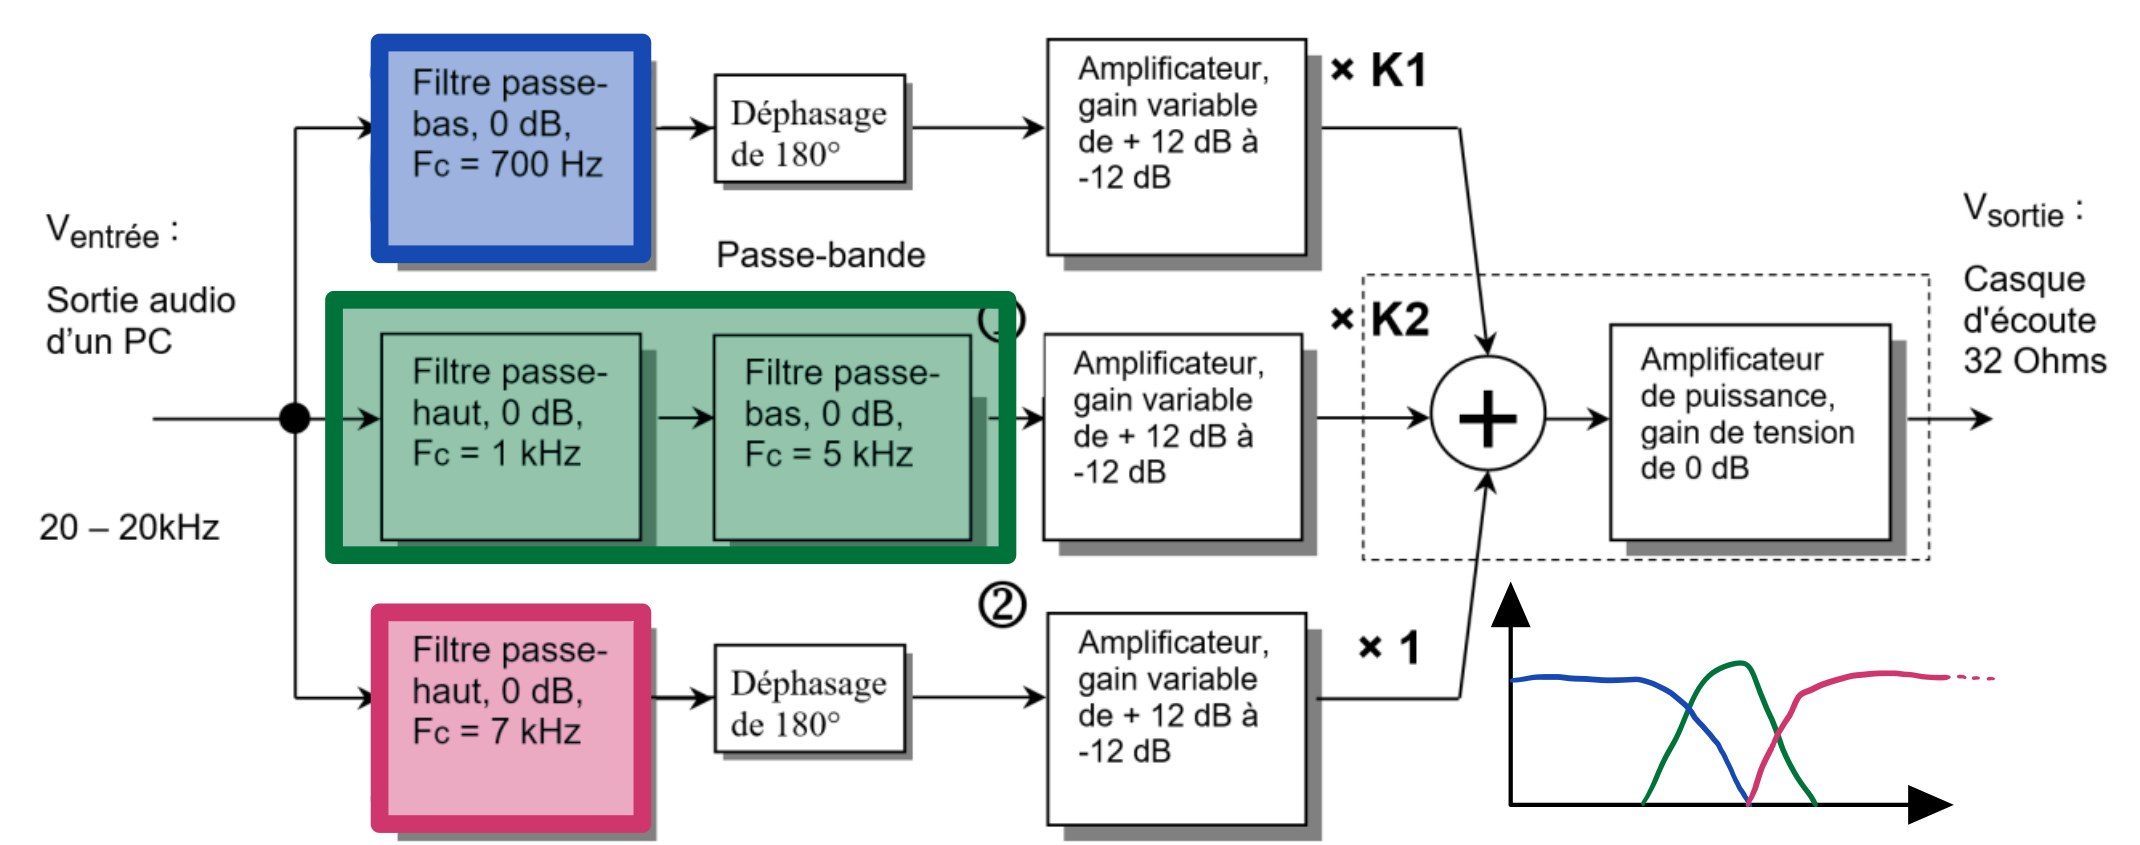
\includegraphics[width=\textwidth]{figure/schema-bloc.png}
    \caption{Schéma bloc du système (un canal)}
  \end{figure}
\end{frame}

\begin{frame}
\frametitle{Idée générale (suite)}
\begin{table}
  \centering
  \caption{Trouvailles faites lors de l'analyse de l'égaliseur}
  \label{tab:wrong-components}
  \begin{tabular}{ll}
    \toprule
    \textbf{Section de circuit fautive} & \textbf{Composante(s) erronée(s)} \\
    \midrule
    \multirow{2}{*}{Assemblement des filtres ($K_1 \& K_2$)} & $R_{11}$ \\
    & $R_{35}$ \\
    \midrule
    \multirow{2}{*}{Filtre passe-haut $f_c=7$ kHz} & $R_{26}$ \\
    & $R_{27}$ \\
    \bottomrule
  \end{tabular}
\end{table}
\end{frame}

\begin{frame}[fragile]
\frametitle{Fonction de transfert python}
\begin{knitrout}\footnotesize
\definecolor{shadecolor}{rgb}{0.969, 0.969, 0.969}\color{fgcolor}\begin{kframe}
\begin{verbatim}
def butterworth(freq, type):
  """
  :param freq: Fréquence de coupure du filtre
  :param type: Type de filtre ('low' ou 'high')
  :return: Coefficients au numérateur et dénominateur du filtre
  """
  wc = 2 * np.pi * freq  # fréquence de coupure rad/s
  b1, a1 = signal.butter(2, wc, type, analog=True)
  return b1, a1
\end{verbatim}
\end{kframe}
\end{knitrout}
\end{frame}

\begin{frame}[fragile]
\frametitle{Attente des buts du client}
\begin{itemize}
  \item Les déphasages naturel des filtres sont correctement corrigés
  \item Le ronflement est atténué par l'utilisation d'Ampli-Op dans nos filtres
\end{itemize}
\end{frame}

\subsection{GEN211: Présentation du lieu de bode}

% TODO: Présentation du lieu de bode CIRCUIT COMPLET CORRIGÉ
%   - [ ] Démontrer comment k1 et k2 sont déterminés (code python?)
%   - [ ] Expliquer pourquoi k1 et k2 rencontrent les spécifications

\begin{frame}[fragile]
% TODO: Print stuff related to K1 and K2
% TODO: Maybe split this in two slides
\frametitle{Validation de $K_1$ et $K_2$}
\begin{knitrout}\footnotesize
\definecolor{shadecolor}{rgb}{0.969, 0.969, 0.969}\color{fgcolor}\begin{kframe}
\begin{verbatim}
k2 = 47.5/60.4
# Passe bande
zp, pp, kp = series_fct(1000, 'high', 5000, 'low')
# Passe Bas
ab, bb = butterworth(700, 'low')
zb, pb, kb = signal.tf2zpk(ab, bb)
# Passe haut
ah, bh = butterworth(7000, 'high')
zh, ph, kh = signal.tf2zpk(ah, bh)
# Combinaison du passe haut et du passe bas
zz, pz, kz = hp.paratf(zb, pb, -kb, zh, ph, -kh)
# Combinaison de la combinaison precedente avec ke pass bande
zt, pt, kt = hp.paratf(zz, pz, kz, zp, pp, kp*k2)
# Fonction de transfert du circuit complet
at, bt = signal.zpk2tf(zt, pt, kt)
\end{verbatim}
\end{kframe}
\end{knitrout}
\end{frame}

\begin{frame}
\frametitle{Réponse en fréquence du circuit complet}
\begin{figure}
\centering % TODO: lieu de bode du circuit complet
\begin{knitrout}\footnotesize
\definecolor{shadecolor}{rgb}{0.969, 0.969, 0.969}\color{fgcolor}
\includegraphics[width=.5\textwidth]{figure/CompleteBodePlot-1} 
\end{knitrout}
\caption{Lieu de bode du circuit complet}
\label{fig:complete-bode}
\end{figure}
\end{frame}


\subsection{GEN211: Analyse des signaux aux points 1 et 2}

% TODO: Calcul des signaux aux points 1 et 2
%   - [ ] explication du raisonnement

\begin{frame}
\frametitle{Analyse des signaux aux points 1}
\footnotesize
\begin{align}
  Y(t)&=0.25\left|H_{1}\right|\cdot\left|H_{2}\right| \sin \left[2 \pi f t+\angle H_{1}+\angle H_{2}\right] \\
  \left|H_{1}\right|&=\frac{\left|-j^{2} \omega^{2}\right|}{\left|j^{2} \omega^{2}+8824 j \omega+3.94 E 9\right|} \\
  \left|H_{1}\right|&=0.989 \\
  \left|H_{2}\right|&=\frac{\left|991102673^{2}\right|}{\left|-\omega^{2}+45044 \omega j+991102673\right|} \\
  \left|H_{2}\right|&=0.965 \\
  \angle H_{1}&=\arctan \left(-j^{2} \omega^{2}\right)-\arctan \left(j^{2} \omega^{2}+8824 j \omega+3.94 E 9\right) \\
  \angle H_{1}&=-2.55 \\
  \angle H_{2}&=\arctan \left(991102673^{2}\right)-\arctan \left(-\omega^{2}+45044 \omega j+991102673\right) \\
  \angle H_{2}&=2.38
\end{align}
\end{frame}

\begin{frame}
\frametitle{Analyse des signaux aux points 2}
\footnotesize
\begin{align}
  Y(s)&=X(s) \cdot H(s) \\
  Y(S)&=\frac{1}{s} \cdot-\frac{s^{2}}{s^{2}+\frac{\omega_{c}}{Q} s+\omega_{c}^{2}} \\
  Y(s)&=-\frac{s}{s^{2}+\frac{\omega_{c}}{Q} s+\omega_{c}^{2}} \\
  Y(t)&=r \cdot e^{-a \cdot t} \cdot \cos (b t+\theta) \cdot u(t) \\
  r&=\sqrt{\frac{\omega_{c}^{2}}{\omega_{c}^{2}-\left(\frac{\omega_{c}}{2 \cdot Q}\right)^{2}}} \\
  b&=\sqrt{\omega_{c}^{2}-\left(\frac{\omega_{c}}{2 \cdot Q}\right)^{2}} \\
  \theta&=\arctan \left(\frac{-\frac{\omega_{c}}{2 \cdot Q}}{-\sqrt{\omega_{c}^{2}-\left(\frac{\omega_{c}}{2 \cdot Q}\right)^{2}}}\right.
\end{align}
\end{frame}

\subsection{GEN230: Pourquoi le filtre et le sommateur sont-ils en erreur?}

% TODO: Présenter étapes importantes du calcul à partir du circuit

\begin{frame}
\frametitle{Erreurs dans le filtre}
\footnotesize
\begin{align}
  \frac{V_{x}-0}{Z_{c}}&=\frac{0-V s}{R_{27}} \\
  V_{x}&=\frac{-V_{s}}{R_{27} \cdot Z_{c}} \\
  \frac{V_{e}-V_{x}}{Z_{c}}&=\frac{V_{x}-V_{s}}{Z_{c}}+\frac{V_{x}}{Z_{c}}+\frac{V_{x}}{R_{26}} \\
  \frac{V_{e}+V_{s}}{Z_{c}}&=V_{x}\left(\frac{3}{Z_{c}}+\frac{1}{R_{26}}\right) \\
  V_{e}+V_{s}&=V_{x}\left(3+\frac{Z_{c}}{R_{26}}\right) \\
  V_{e}+V s&=V_{x}\left(3+\frac{1}{s \cdot c \cdot R_{26}}\right) \\
  V_{e}&=V_{x}\left(3+\frac{1}{s \cdot c \cdot R_{26}}+R_{27} \cdot s \cdot C\right) \\
  V_{s}&=-V_{x} \cdot s \cdot C \cdot R_{27} \\
\end{align}
\end{frame}

\begin{frame}
\frametitle{Erreurs dans le filtre (suite)}
\begin{align}
  H(s)&=\frac{V_{s}}{V_{e}}=\frac{-V_{x} \cdot s \cdot C \cdot R_{27}}{V_{x}\left(3+\frac{1}{s \cdot c \cdot R_{26}}+R_{27} \cdot s \cdot C\right)} \\
  H(s)&=\frac{-s^{2}}{s^{2}+\frac{3 \cdot s}{C \cdot R_{27}}+\frac{1}{R_{26} \cdot R_{27} \cdot C^{2}}} \\
  \frac{3}{C \cdot R_{27}}&=\frac{\omega_{0}}{Q} \\
  Q&=0.707 \\
  \frac{1}{R_{26} \cdot R_{27} \cdot C^{2}}&=w_{0}^{2} \\
  R_{27}&=\frac{3 \cdot Q}{C \cdot \omega_{0}} \\
  R_{26}&=\frac{1}{\omega_{0}^{2} \cdot R_{27} \cdot C^{2}}
\end{align}
\end{frame}

\begin{frame}
\frametitle{Erreurs dans le sommateur}
\begin{align}
  \frac{ R_{71} }{R_{35}} &= 1  \Rightarrow R_{71} = R_{35} \\
  R_{71} &= \SI{47.5}{\kilo\ohm} \Rightarrow R_{35} = \SI{47.5}{\kilo\ohm} \\
  K_1 &= 1 \textrm{(Déterminé de façon expérimentale)} \\
  K_1 &= \frac{R_{71}}{R_{11}} = 1 \Rightarrow R_{11} = R_{71} = \SI{47.5}{\kilo\ohm} \\
  R_{25} &= \SI{60.4}{\kilo\ohm} \\
  K_2 &= \frac{R_{71}}{R_{25}} \Rightarrow K_2 = \frac{47.5}{60.4} = 0.79 \\
\end{align}
\end{frame}

\section{Observations expérimentales}

\subsection{GEN211: Code python en temps réel}

% TODO: Filtre corrigé
%   - [ ] Poles et zeros
%   - [ ] Lieu de bode
%   - [ ] Délai de groupe (incluant bon k1 et k2 + gains des 3 filtres 0dB)

\begin{frame}
\frametitle{Filtre corrigé}
\begin{figure}
\centering
\begin{knitrout}\footnotesize
\definecolor{shadecolor}{rgb}{0.969, 0.969, 0.969}\color{fgcolor}
\includegraphics[width=.5\textwidth]{figure/PolesZerosFilter-3} 
\end{knitrout}
\caption{Pôles et zéros du filtre corrigé}
\label{fig:poles-zeros-filter}
\end{figure}
\end{frame}

\begin{frame}
\frametitle{Filtre corrigé (suite)}
\begin{figure}
\centering
\begin{knitrout}\footnotesize
\definecolor{shadecolor}{rgb}{0.969, 0.969, 0.969}\color{fgcolor}
\includegraphics[width=.5\textwidth]{figure/BodeCorrectedPlot-5} 
\end{knitrout}
\caption{Lieu de Bode du filtre corrigé}
\label{fig:bode-filter}
\end{figure}
\end{frame}

\begin{frame}
\frametitle{Délai de groupe du filtre corrigé}
\begin{figure}
\centering
\begin{knitrout}\footnotesize
\definecolor{shadecolor}{rgb}{0.969, 0.969, 0.969}\color{fgcolor}
\includegraphics[width=.5\textwidth]{figure/DelayCorrectedPlot-7} 
\end{knitrout}
\caption{Délai de groupe du filtre corrigé}
\label{fig:delay-corrected}
\end{figure}
\end{frame}

\subsection{GEN211: Simulation Altium du filtre corrigé}

% TODO: Simulation Altium
%   - [ ] Lieu de bode
%   - [ ] Monte Carlo

\begin{frame}
\frametitle{Simulations Altium du filtre corrigé}
\begin{figure}
\centering
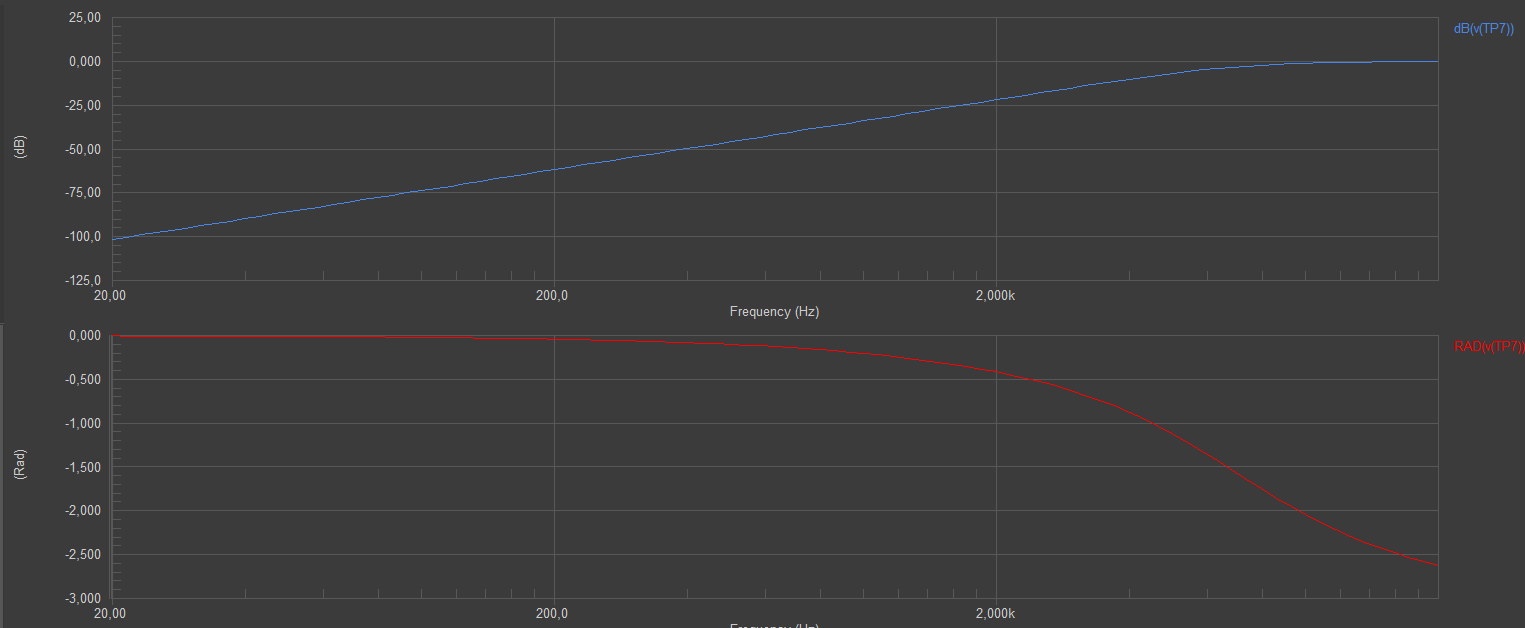
\includegraphics[width=.8\textwidth]{figure/altium-bode-filter.png}
\caption{Lieu de bode du filtre corrigé}
\label{fig:altium-bode-filter}
\end{figure}
\end{frame}

\begin{frame}
\frametitle{Simulations Altium du filtre corrigé (suite)}
\begin{figure}
\centering
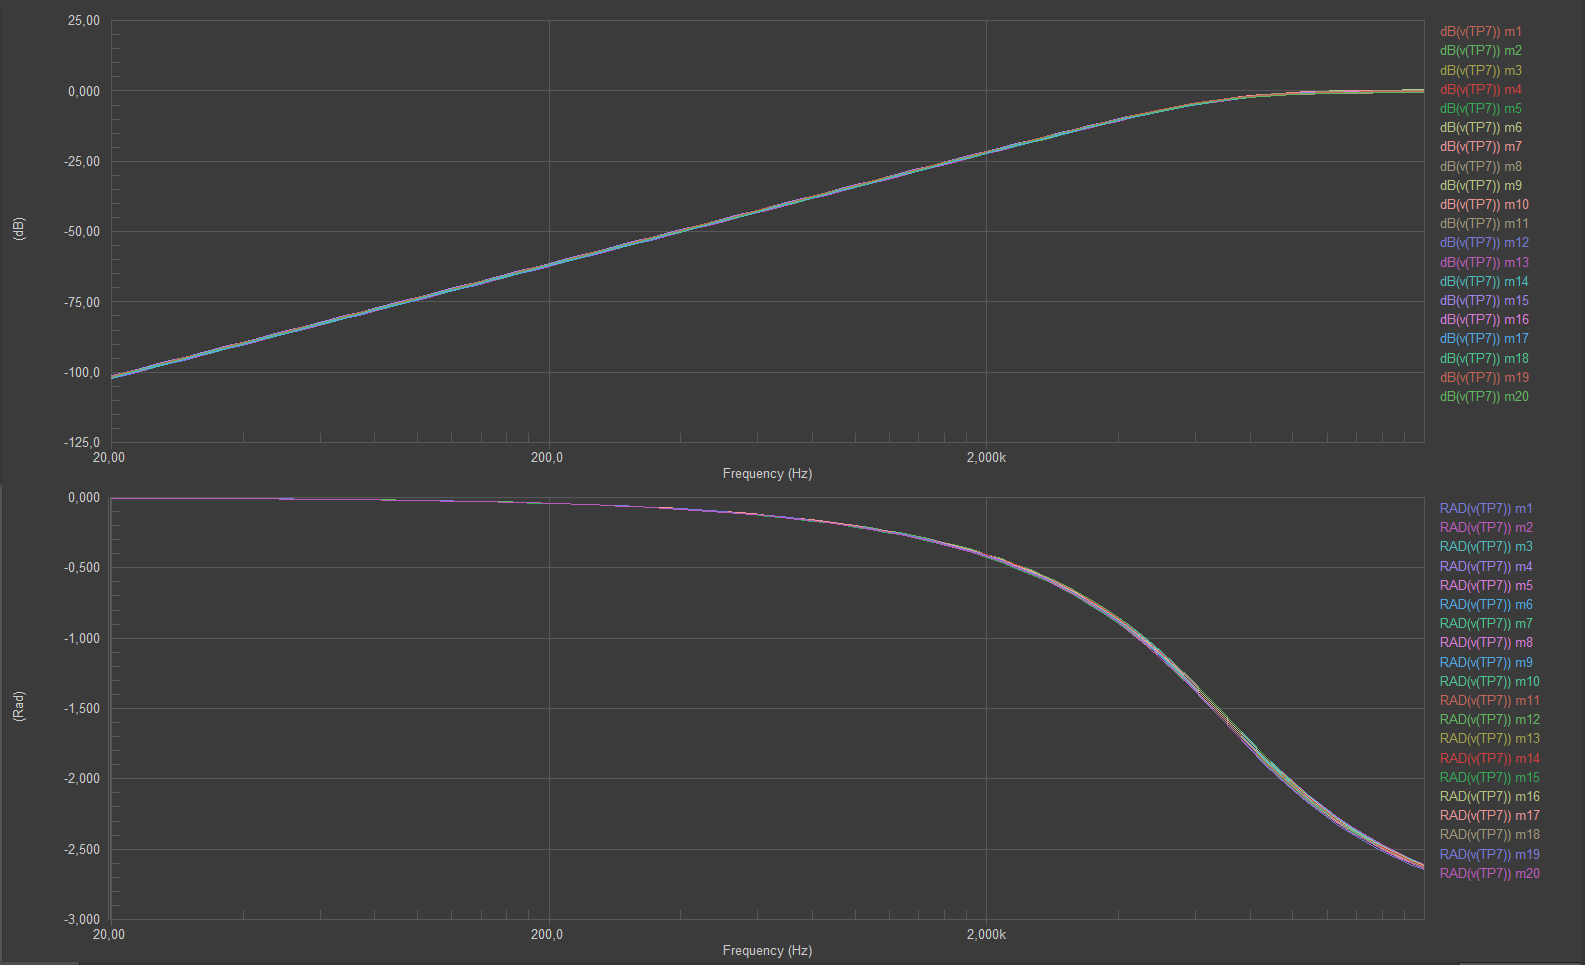
\includegraphics[width=.8\textwidth]{figure/altium-monte-carlo-filter.png}
\caption{Simulation Monte Carlo du filtre corrigé}
\label{fig:altium-monte-carlo-filter}
\end{figure}
\end{frame}


\subsection{GEN211: Simulation Altium du circuit complet corrigé}

% TODO: Simulation Altium
%   - [ ] Lieu de bode
%   - [ ] Délai de groupe à la sortie

\begin{frame}
\frametitle{Simulations Altium du circuit complet corrigé}
\begin{figure}
\centering
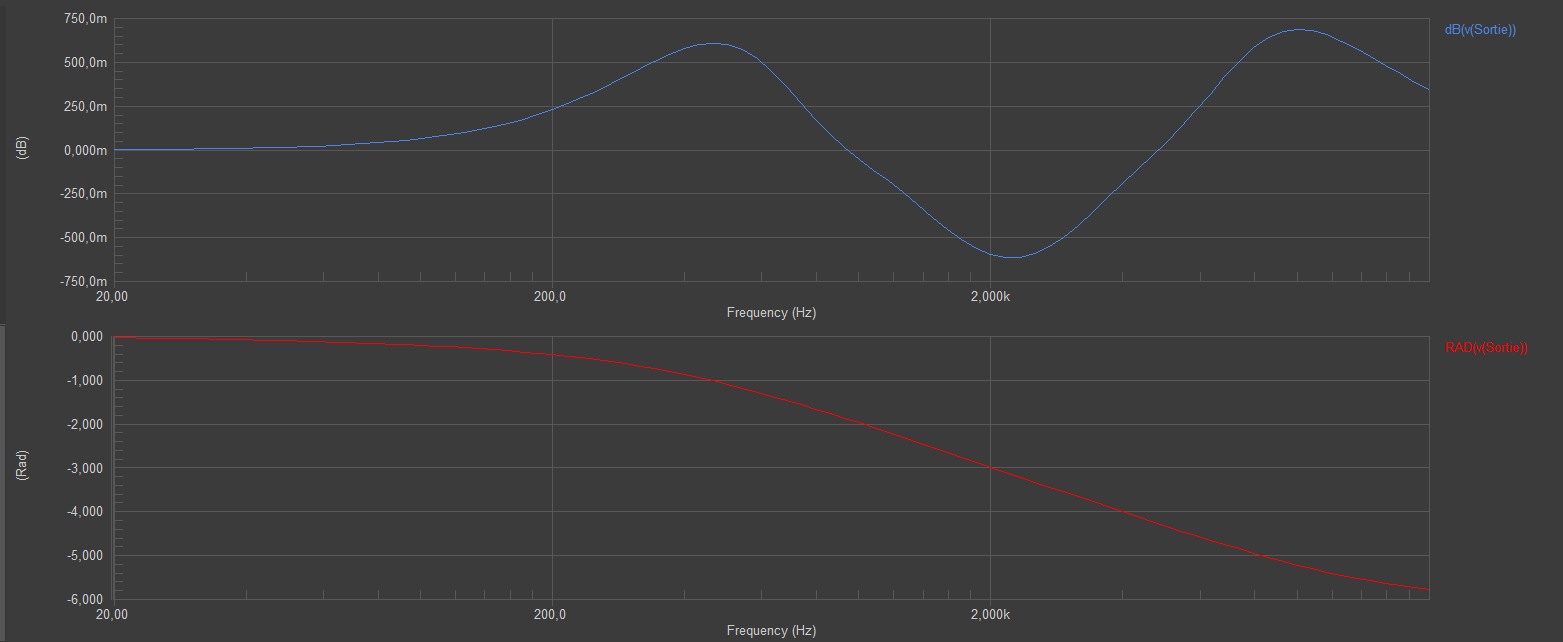
\includegraphics[width=.8\textwidth]{figure/altium-bode-complete.png}
\caption{Lieu de bode du circuit complet corrigé}
\label{fig:altium-bode-complete}
\end{figure}
\end{frame}

\begin{frame}
\frametitle{Simulations Altium du circuit complet corrigé (suite)}
\begin{figure}
\centering
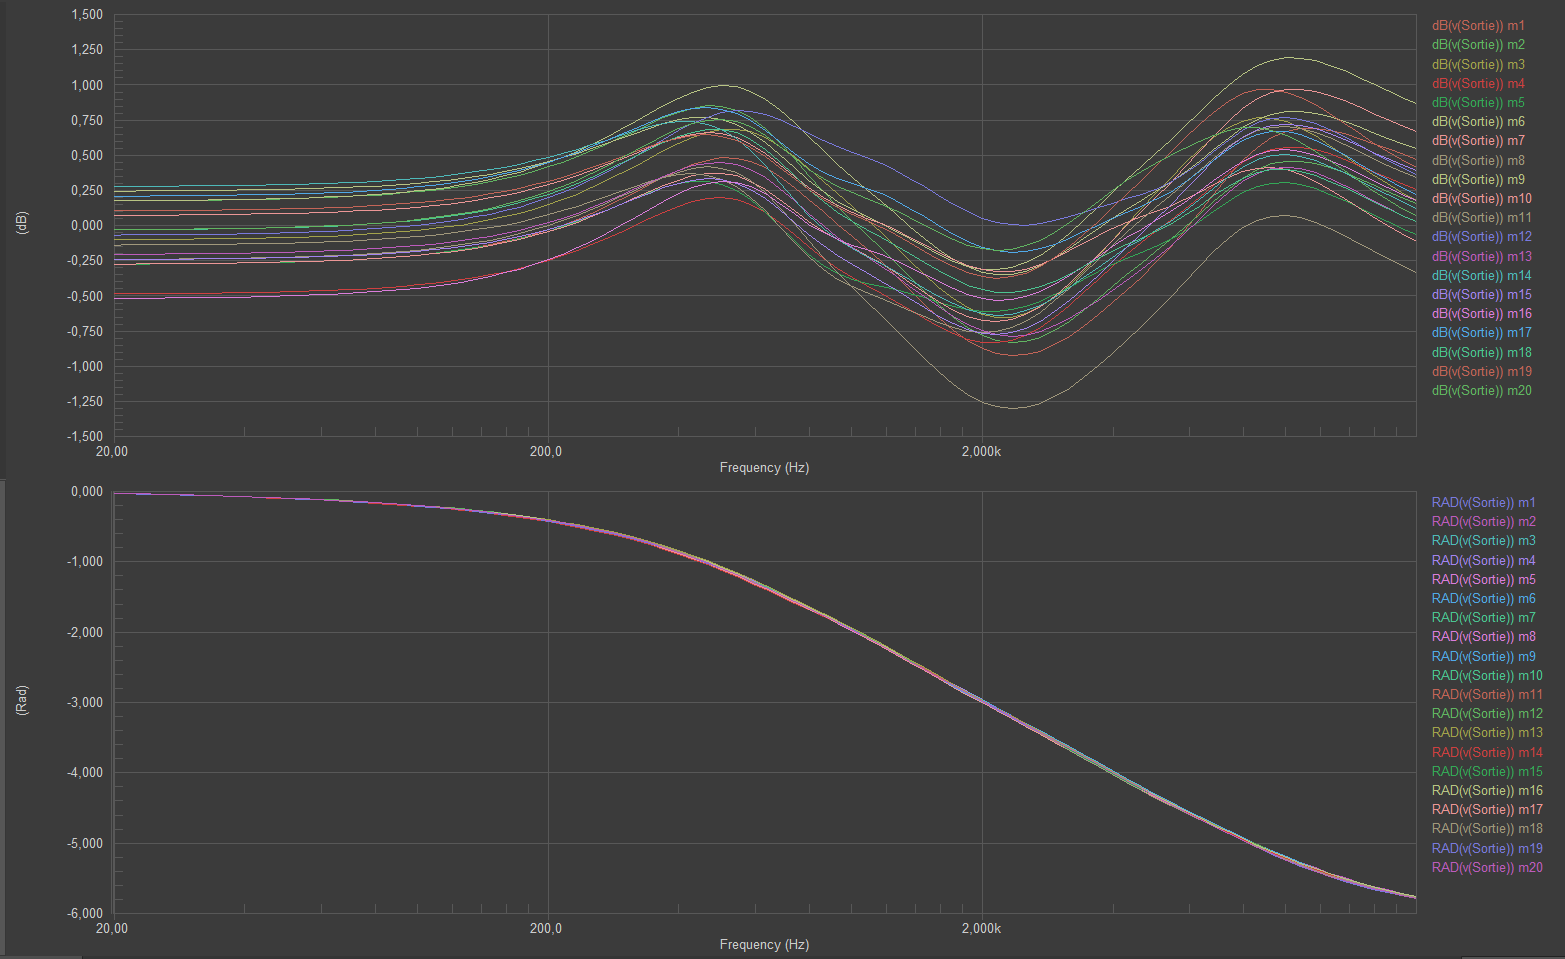
\includegraphics[width=.8\textwidth]{figure/altium-monte-carlo-complete.png}
\caption{Simulation Monte Carlo du filtre corrigé}
\label{fig:altium-monte-carlo-complete}
\end{figure}
\end{frame}


% \section{Slides non-triées TODO: à trier}
%
% \begin{frame}
%   \frametitle{Papier 3}
%   \begin{align}
%     \frac{V_x-0}{R_2} &= \frac{0-V_s}{2C_3} \\
%     \frac{V_x}{R_2} &= \frac{-V_s}{2C_3} \\
%     V_x &= \frac{-V_sR_2}{2C_3} \\
%     \frac{V_e - V_x}{R} &= \frac{V_x - V_s}{R} + \frac{V_x}{Z_{C_2}} + \frac{V_x}{R_2} \\
%     \frac{V_e}{R} &= \frac{2V_x}{R} - \frac{V_s}{R} + \frac{V_x}{Z_{C_2}} + \frac{V_x}{R_2} \\
%     % XXX: C'est quoi qui est réellement ecrit au R/R ?
%     \frac{V_e}{R} &= V_x \left( \frac{2}{R} + \frac{1}{Z_{C_2}} + \frac{1}{R_2} \right) - \frac{V_s}{R} \\
%     V_e + V_s &= R V_x \left( \frac{2}{R} + \frac{1}{Z_{C_2}} + \frac{1}{R_2} \right)
%   \end{align}
% \end{frame}
%
% \begin{frame}
%   \frametitle{Papier 4}
%   \begin{align}
%     V_e &= RV_x \left( \frac{2}{R} + \frac{1}{R_2} + \right) \\
%     V_s &= \frac{-V_xZ_{C_3}}{R_2} \\
%     % XXX: 2/R ou 1/R (premiere frac du \left( \right) )?
%     H &= \frac {\frac{-1}{R_2sC_3} }{
%            R\left(\frac{2}{R}+\frac{1}{R_2}+\frac{sC_2}{1}\right)+\frac{1}{R_2sC_3}
%          } \\
%     H &= \frac{1}{ RR_2sC_3 + \left(\frac{2}{R} + \frac{1}{R_2} + sC_2\right)+1 } \\
%     H &= \frac{1}{s\left[(R_2+2R)C_3\right]+R R_2 C_2 C_3 s^2 +1} \\
%     H &= \frac{\frac{1}{R R_2 C_2 C_3}}{
%       s^2 + s\left[\frac{R_2 + 2R}{R R_2 C_2}\right]+\frac{1}{R R_2 C_2 C_3}
%     }
%   \end{align}
% \end{frame}

\end{document}
